\documentclass{astroedu-lab}

\begin{document}

\pagestyle{plain}

\begin{problem}{\huge Лабораторная работа 2.4.1\\\\Определение теплоты испарения\\\\жидкости\\\\Выполнил Жданов Елисей Б01-205}

\section{Цель работы:}

1) Измерение давления насыщенного пара жидкости при разной температуре

2) Вычисление по полученным данным теплоты испарения с помощью уравнения Клапейрона–Клаузиуса

\section{Оборудование:}

Термостат

Герметический сосуд, заполненный исследуемой жидкостью

Отсчетный микроскоп

\section{Теоретическая справка}

Для определения теплоты испарения будет использован косвенный метод, основанный на формуле Клапейрона–Клаузиуса.

\begin{equation}
	\frac{d P}{d T}=\frac{L}{T\left(V_2-V_1\right)}
\end{equation}

Вследствие высокой плотности воды положим изменение объемов равным(считая при атмосферном давлении пар идеальным газом).

\begin{equation}
	V=\frac{R T}{P}
\end{equation}

Подставляя выражение в уравнение Клапейрона–Клаузиуса, получим

\begin{equation}
	\boxed{L=\frac{R T^2}{P} \cdot \frac{d P}{d T}=-R \frac{d(\ln P)}{d(1 / T)}}
\end{equation}

Буду строить зависимость ln(P) от 1/T для нахождения L из коэффициента наклона прямой

\section{Экспериментальная установка}

\begin{figure}[!h]
	\centering
	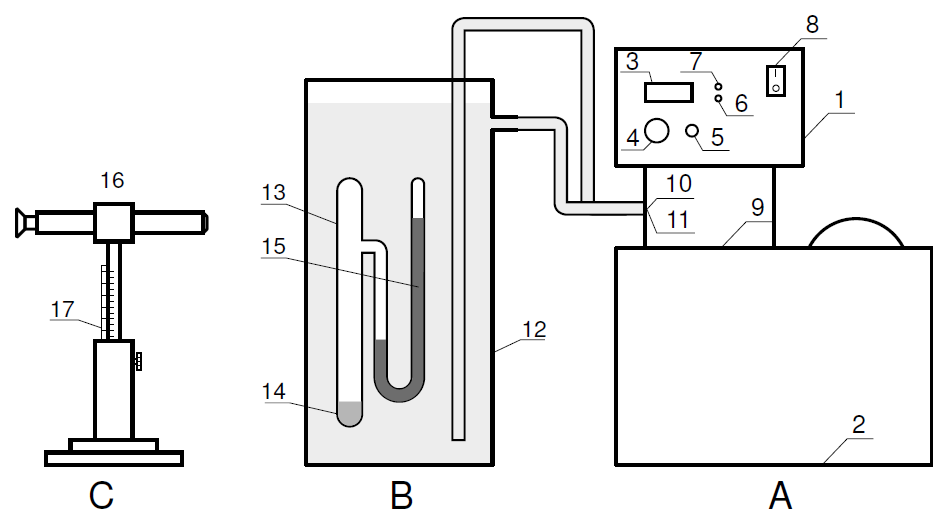
\includegraphics[width=0.9\textwidth]{установка.png}
	\label{fig:boiler}
\end{figure}

Над ртутью находится насыщенный пар (перед заполнением прибора воздух из него был откачан). Давление насыщенного пара определяется по манометру, соединенному с исследуемым объемом.

\section{Измерения, Обработка}

1) Разность уровней в манометре:

\begin{equation}
	\Delta h = 29.59 + 7.92 = (37.51 \pm 0.09) \text{ мм. рт. ст.}
\end{equation}

Температура в наччальный момент

\begin{equation}
	T = 20.16 ^\circ C
\end{equation}

2) Запишем показания приборов при нагреве жидкости

\begin{center}
\begin{tabular}{|c|c|}
\hline 
T, $^\circ$C  & $h_1$, мм\\
\hline
20.16 & 0.00 \\
22.32 & 2.86 \\
24.30 & 5.91 \\
26.30 & 9.22 \\
28.26 & 12.78 \\
30.26 & 16.63 \\
32.24 & 20.95 \\
34.23 & 25.72 \\
36.23 & 30.88 \\
38.22 & 36.28 \\
40.22 & 42.08 \\
\hline
\end{tabular}
\end{center}

Аналогично охлаждение

\begin{center}
\begin{tabular}{|c|c|}
\hline 
T, $^\circ$C  & $h_1$, мм\\
\hline
40.22 & 42.08 \\
38.05 & 35.78 \\
36.02 & 30.52 \\
34.09 & 25.58 \\
32.04 & 20.56 \\
30.02 & 16.51 \\
28.02 & 12.33 \\
26.02 & 9.16 \\
23.96 & 5.81 \\
22.25 & 2.85 \\
20.12 & 0.09 \\
\hline
\end{tabular}
\end{center}

4) Формула для пересчета давления

\begin{equation}
	\Delta P = \rho g (x_2^{(0)} - x_2^{(0)} + 2(x_2 - x_2^{(0)}))
\end{equation}

При калибровке прибора

\begin{equation}
	x_2^{(0)} = 0
\end{equation}

Поэтому

\begin{equation}
	\Delta P = \rho g (\Delta h + 2 x_2)
\end{equation}

4) Построю 2 графика соответствующие нагреву и охлаждению

\begin{figure}[!h]
	\centering
	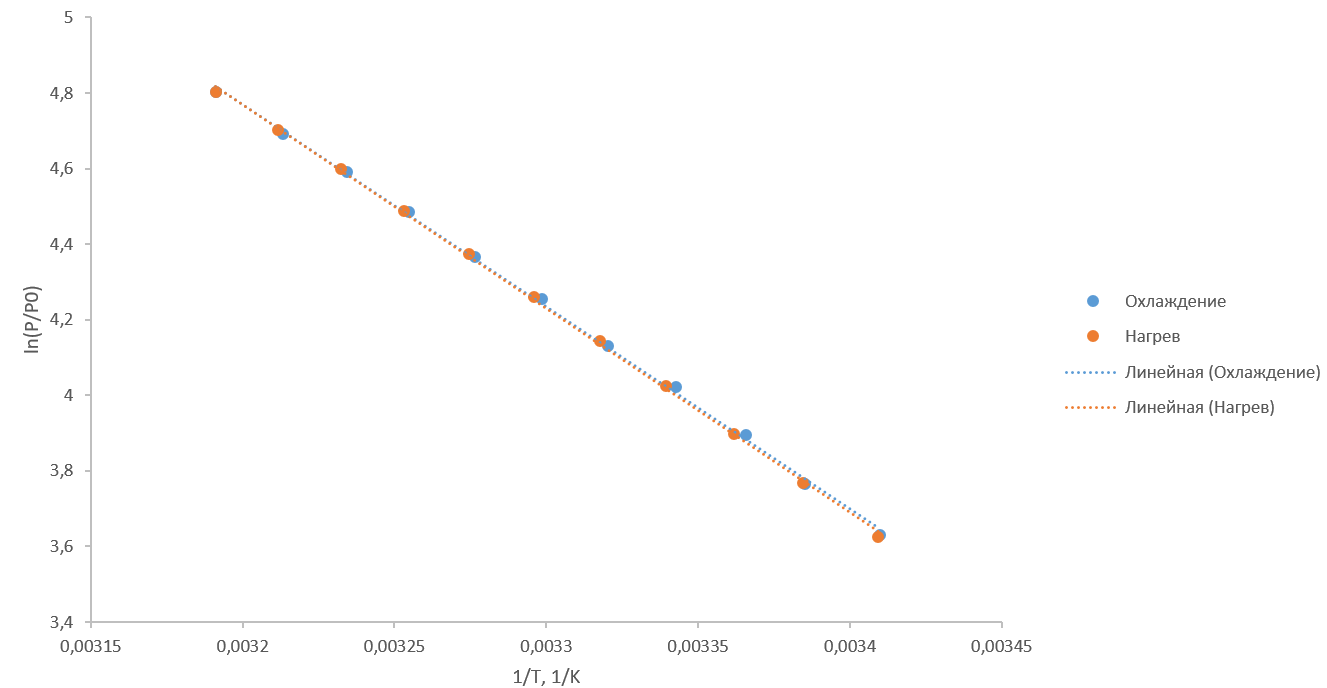
\includegraphics[width=1\textwidth]{график.png}
	\label{fig:boiler}
\end{figure}

Буду строить зависимость $ln(P/P_0)$ от 1/T для нахождения L из коэффициента наклона прямой, принимая за $P_0$ величину $\rho g$

Аппроксимация МНК для нагрева

\begin{equation}
	y = (22.04 \pm 0.14) - (5398 \pm 44) \cdot x
\end{equation}

Для охлаждения

\begin{equation}
	y = (21.90 \pm 0.18) - (5352 \pm 55) \cdot x
\end{equation}

\[
	a = \frac{<x_i y_i> - < x > < y_i >}{< x_i^2> - < x_i >^2}
\]

\[
	b = < \nu_i > - a < N_i >
\]

Их погрешности

\begin{equation}
	S_a^2 = \frac{< x_i^2>}{< x_i^2 > - < x_i >^2} \cdot \frac{<  b_i - b > ^2}{n - 2}
\end{equation}

Соответствующие L нагрева

\begin{equation}
	L_\text{нагр} = (44900 \pm 400) \frac{\text{Дж}}{\text{моль}}
\end{equation}

Охлаждения

\begin{equation}
	L_\text{охл} = (44500 \pm 500) \frac{\text{Дж}}{\text{моль}}
\end{equation}

\section{Вывод}

Как видно, точность измерений при охлаждении получается ниже, чем при нагреве. Сам процесс замера при охлаждении более сложен по сравнению с нагревом, поскольку из-за гистерезиса выпуклости поверхностного натяжения на конце ртути сложно правильно находить манометрическую высоту столба. Поэтому при охлаждении были попытки проводить измерения, сначала опуская температуру немного ниже положенной, с последующим подогревом для образования устойчивой постоянной выпуклости. Также очевидно, что точность определяется характеристиками манометра, а значит почти не связана с теоретической методикой.

Тем не менее, результаты согласуются в пределах погрешностей.

Табличная молярная теплота парообразования спирта составляет 41800 Дж/моль.

\section{Ресурсы}

Расчет по МНК: метод-наименьших-квадратов.рф

\end{problem}
\end{document}